\documentclass[a4paper,11pt]{article}

\usepackage[utf8]{inputenc}
\usepackage[left=1in,right=1in,top=1in,bottom=1in]{geometry}
\usepackage{amsmath,amssymb,amsfonts,bm}
\usepackage{pgfplots,graphicx,calc,changepage,caption}
\pgfplotsset{compat=newest}
\usepackage{enumitem}
\usepackage{fancyhdr, titling, titlesec}
\usepackage[colorlinks = true, linkcolor = cyan]{hyperref}

\DeclareMathOperator{\sech}{sech}
\DeclareMathOperator{\csch}{csch}
\DeclareMathOperator{\arcsec}{arcsec}
\DeclareMathOperator{\arccot}{arcCot}
\DeclareMathOperator{\arccsc}{arcCsc}
\DeclareMathOperator{\arccosh}{arcCosh}
\DeclareMathOperator{\arcsinh}{arcsinh}
\DeclareMathOperator{\arctanh}{arctanh}
\DeclareMathOperator{\arcsech}{arcsech}
\DeclareMathOperator{\arccsch}{arcCsch}
\DeclareMathOperator{\arccoth}{arcCoth} 
\newcommand{\nats}{\mathbb{N}}
\newcommand{\reals}{\mathbb{R}}
\newcommand{\rats}{\mathbb{Q}}
\newcommand{\ints}{\mathbb{Z}}
\newcommand{\pols}{\mathcal{P}}
\newcommand{\cants}{\Delta\!\!\!\!\Delta}
\newcommand{\eps}{\varepsilon}
\newcommand{\st}{\backepsilon}
\newcommand{\abs}[1]{\left| #1 \right|}
\newcommand{\dom}[1]{\mathrm{dom}\left(#1\right)}
\newcommand{\for}{\text{ for }}
\newcommand{\dd}[1]{\mathrm{d}#1}
\newcommand{\spn}{\mathrm{sp}}
\newcommand{\nul}{\mathcal{N}}
\newcommand{\col}{\mathrm{col}}
\newcommand{\rank}{\mathrm{rank}}
\newcommand{\norm}[1]{\lVert #1 \rVert}
\newcommand{\inner}[1]{\left\langle #1 \right\rangle}
\newcommand{\pmat}[1]{\begin{pmatrix} #1 \end{pmatrix}}
\renewcommand{\and}{\text{ and }}
\newcommand{\bigO}{\mathcal{O}}

% Common bold symbols
\newcommand{\bx}{\mathbf{x}}
\newcommand{\bl}{\pmb{\lambda}}
\newcommand{\bF}{\mathbf{F}}

\newsavebox{\qed}
\newenvironment{proof}[2][$\square$]
    {\setlength{\parskip}{0pt}\par\textit{Proof:} #2\setlength{\parskip}{0.25cm}
        \savebox{\qed}{#1}
        \begin{adjustwidth}{\widthof{Proof:}}{}
    }
    {
        \hfill\usebox{\qed}\end{adjustwidth}
    }

\pagestyle{fancy}
\fancyhead{}
\lhead{Caleb Jacobs}
\chead{RBF Interpolants Over Near-Flat Surfaces}
\rhead{27 April 2022}
\cfoot{}
\setlength{\headheight}{35pt}
\setlength{\parskip}{0.25cm}
\setlength{\parindent}{0pt}
\titleformat*{\section}{\Large\bfseries}

\setlength{\droptitle}{-10em}
\title{RBF Interpolants Over Near-Flat Surfaces}
\author{Caleb Jacobs}
\date{27 April 2022}

\begin{document}
\maketitle
\thispagestyle{empty}

\begin{abstract}
	\noindent
	In the context of smooth radial basis function (RBF) based methods, utilizing the collocation matrix with a small shape parameter is desirable. A small shape parameter tends to increase accuracy of RBF interpolants or finite difference weights. To properly resolve systems with a small shape parameter, methods such as RBF-RA are used. Methods such as RBF-RA work great for data that is on a flat surface or a curved surface. However, applying RBF-RA to data that is on a near-flat surface leads to erroneous results. We present results based on asymptotology and perturbation theory to better understand these erroneous results. Furthermore, we present current, in-progress research to again further this understanding.
\end{abstract}

\section{Background}
In the context of data interpolation, finite differences, and an abundance of many other data driven problems, radial basis function (RBF) based methods are becoming more and more popular due to there flexibility and high orders of accuracy. An RBF is any radially symmetric function $ \phi_\eps(r) $ where $ \eps $ is called the shape parameter. For this article, we will focus on smooth RBFs and even more specifically, we will only consider the GA RBF in \autoref{table:RBFs}. As mentioned before, RBFs can be used as a general interpolation basis which we will consider next.

\begin{table}[t]
	\captionsetup{width = 0.57\linewidth}
	\caption{Commonly used, smooth radial basis functions.}
	\[
	\begin{array}{ll}
		\hline \\[-2ex]
		\text{RBF Name} & \text{Radial function } \phi(r) \\
		\hline \\[-2ex]
		\text{Gaussian (GA)} & \phi_\eps(r) = e^{-(\eps r)^2} \\
		\text{Multiquadric (MQ)} & \phi_\eps(r) = \sqrt{1 + (\eps r)^2} \\
		\text{Inverse Multiquadric (IMQ)} & \phi_\eps(r) = 1 / \sqrt{1 + (\eps r)^2} \\
		\text{Inverse Quadratic (IQ)} & \phi_\eps(r) = 1 / (1 + (\eps r)^2) \\
		\text{Sech (SH)} & \phi_\eps(r) = \sech(\eps r) \\
		\hline
	\end{array}
	\]
	\label{table:RBFs}
\end{table}

Suppose we have data $ \{\bx_i, f_i\}_{i = 1}^n $ that we would like to interpolate using RBFs. Then, an RBF interpolant of the data can be written as

\begin{equation}
	s(\bx) = \sum_{i = 1}^n \lambda_i \phi_\eps (\norm{\bx - \bx_i}_2) \label{equ:interp}
\end{equation}

where $ \lambda_i $ are the interpolation weights. This interpolant is incomplete in that we still need to determine each $ \lambda_i $. A linear system for $ \lambda_i $ is given by

\begin{equation}
	\underbrace{\pmat{
			\phi_\eps (\norm{\mathbf{x}_1 - \mathbf{x}_1}) & \phi_\eps (\norm{\mathbf{x}_1 - \mathbf{x}_2}) & \cdots & \phi_\eps (\norm{\mathbf{x}_1 - \mathbf{x}_n}) \\
			\phi_\eps (\norm{\mathbf{x}_2 - \mathbf{x}_1}) & \phi_\eps (\norm{\mathbf{x}_2 - \mathbf{x}_2}) & \cdots & \phi_\eps (\norm{\mathbf{x}_2 - \mathbf{x}_n}) \\
			\vdots & \vdots & \ddots & \vdots \\
			\phi_\eps (\norm{\mathbf{x}_n - \mathbf{x}_1}) & \phi_\eps (\norm{\mathbf{x}_n - \mathbf{x}_2}) & \cdots & \phi_\eps (\norm{\mathbf{x}_n - \mathbf{x}_n})
	}}_{A} \underbrace{\pmat{
			\lambda_1 \\ \lambda_2 \\ \vdots \\ \lambda_n
	}}_{\pmb{\lambda}} = \underbrace{\pmat{
			f_1 \\ f_2 \\ \vdots \\ f_n
	}}_{\bF} \label{equ:direct}
\end{equation}

where $ A $ is known as the collocation matrix. A known property of smooth RBF interpolants is that decreasing the shape parameter $ \eps $ will increase the accuracy of the interpolant. Thus, we would like to solve \eqref{equ:direct} for small $ \eps $. However, decreasing $ \eps $ will quickly lead to a very ill-conditioned collocation matrix \cite{rbf}. Solving \eqref{equ:direct} using a standard linear solve function in your preferred language is known as RBF-Direct; RBF-Direct greatly suffers from the small $ \eps $ ill-conditioning of $ A $. Instead, we will solve $ \eqref{equ:direct} $ using an indirect method that leverages properties of the GA RBF and some other smooth RBFs. 

One of the most important properties of the GA RBF is that it is complex analytic. This analyticity of GA means we can use contour integration in $ \eps $ in a well conditioned regime to stably resolve GA interpolants for small $ \eps $. The idea is to pick points to evaluate our interpolant at and then put the interpolants in an analytic vector function of $ \eps $ denoted by $ \mathbf{s}(\eps) $. Then, using Cauchy's integral formula, we have
\[
	\mathbf{s}(\eps) = \frac{1}{2\pi i} \oint_\Gamma \frac{\mathbf{s}(z)}{z - \eps} \dd z
\] 
where $ \Gamma $ is a counterclockwise oriented circle with center at $ \eps $. The radius of $ \Gamma $ is ideally picked so that evaluation of the integrand on the contour is at values of $ \eps $ such that the collocation matrix is well-conditioned. 

The first method to use contour integration to evaluate RBF interpolants is know as RBF Contour-Pad\'e (RBF-CP). RBF-CP utilizes Pad\'e approximates to construct a rational approximation that we then apply contour integration to. Pad\'e approximations work alright but there are a few pitfalls with stability and finding poles of the approximation \cite{rbf-ra}. A recent successor to RBF-CP is know as RBF-RA where the RA stands for rational approximation. RBF-RA differs from RBF-CP in that the rational vector approximation is now constructed to be a more general rational function with the poles being easily accessible. RBF-RA appears to work great most of the time but fails in some unexpected cases.

Applying RBF-RA to data that lies on a completely flat surface (i.e. a plane) gives stable and desired results. Similarly, RBF-RA applied to data that lies on a relatively curvy surface also works well. Yet, interestingly, applying RBF-RA to data that lies on a near-flat surface yields erroneous and unusable results! The instability of RBF-RA for near-flat data is unexpected because it works well in both limiting cases (i.e. completely flat and non-flat data). We wish to explore the so called near-flat surface limit of the RBF interpolation problem. 


\section{Flat surface perturbations of the collocation matrix}

To study the near-flat surface limit, we need to construct some data on a near flat surface. One of the simplest near-flat surfaces is a sphere with small curvature $ \kappa $ and top of the sphere centered at the origin; the sphere described is given by
\begin{equation}
	x^2 + y^2 + \left(z + \frac{1}{\kappa}\right)^2 = \frac{1}{\kappa^2}, \quad 0 < \kappa \ll 1. \label{equ:sphere}
\end{equation}
We can then construct data satisfying \eqref{equ:sphere}. Suppose we have $ n $ distinct $ x $-$ y $ pairs of data $ \{x_i, y_i\}_i^n $ scattered over the unit disk. Then, define our nodes or data set $ \{\bx_i\}_i^n $ satisfying \eqref{equ:sphere} as
\begin{equation}
	\bx_i = \left\langle x_i, y_i, \sqrt{\frac{1}{\kappa^2} - r_i^2} - \frac{1}{\kappa} \right\rangle \label{equ:data}
\end{equation}
where the radii $ r_i $ from the origin are given as
\[
	r_i = \sqrt{x_i^2 + y_i^2}.
\]
It is worth mentioning that the nodes defined in \eqref{equ:data} are just points in the $ x $-$ y $ plane projected down onto the sphere described in \eqref{equ:sphere}. Example node sets can be seen in \autoref{plot:data}.

\begin{figure}[t]
	\centering
	\captionsetup{width = 0.9\textwidth}
	\caption{Sample of 64 nodes generated using \eqref{equ:data} for various curvatures. Note, RBF-RA works well for data in the left and right plots but struggles with data in the middle plot.}
	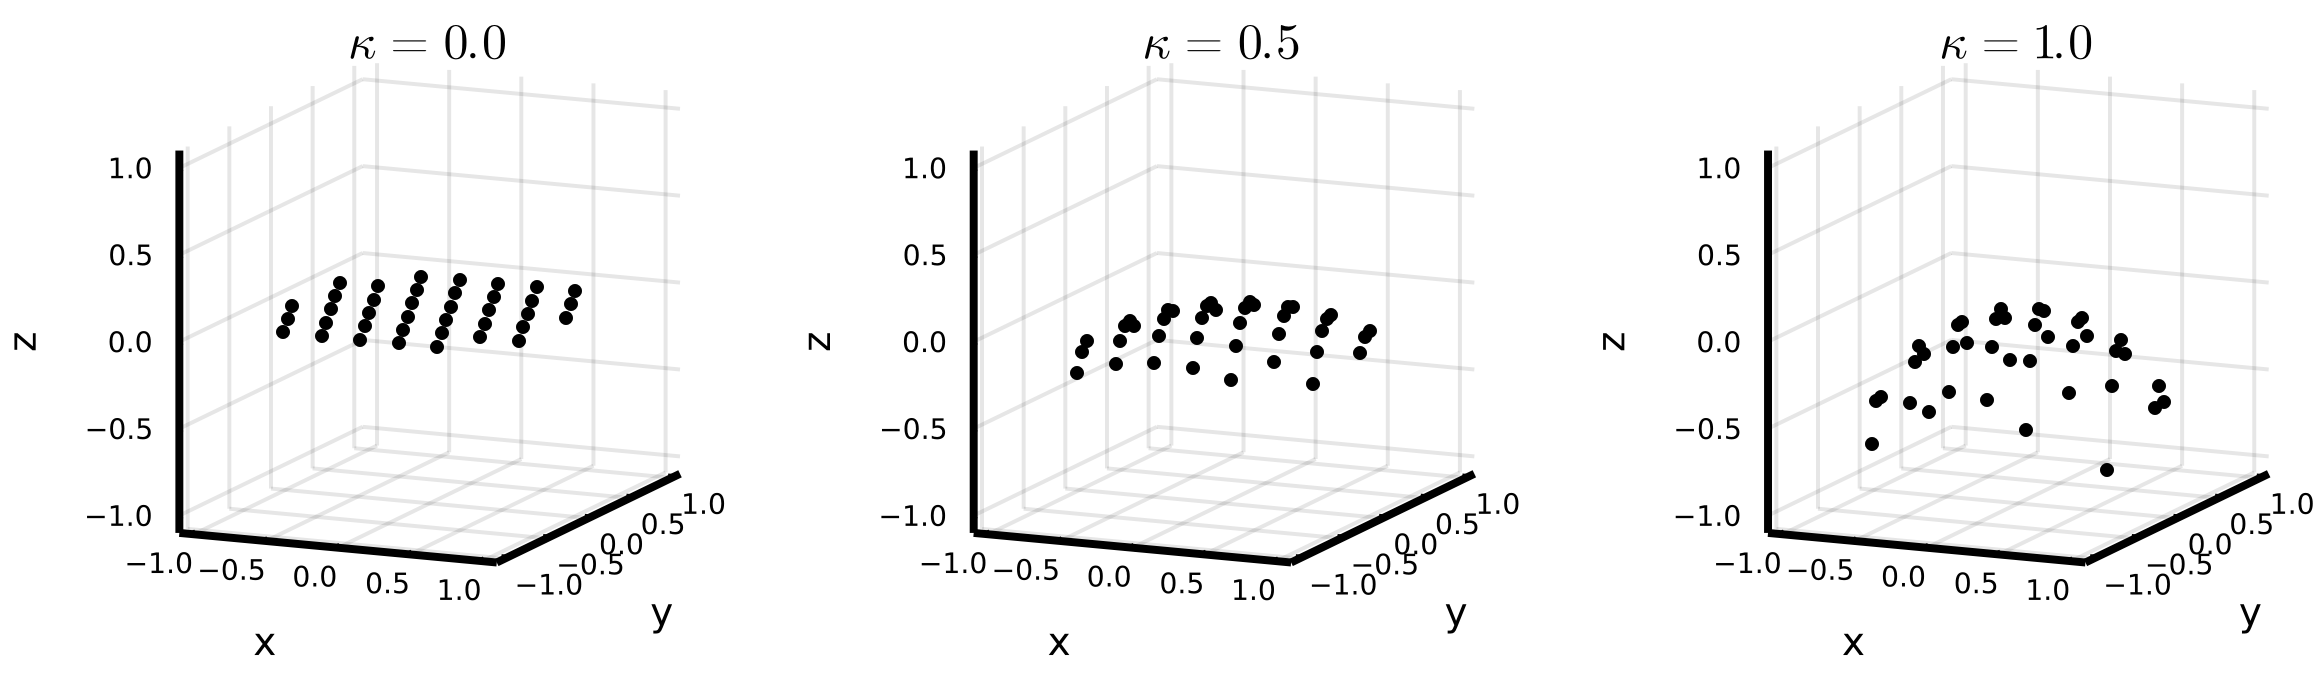
\includegraphics[width = 0.9\textwidth]{Images/Nodes.png}
	\label{plot:data}
\end{figure} 

With $ \kappa $ dependent nodes defined, we now seek to understand how the collocation matrix behaves with $ \kappa $. To construct the collocation matrix, we need to compute all pairwise differences in our node set. By direct computation with \eqref{equ:data}, we have
\begin{equation}
	\norm{\bx_i - \bx_j}_2^2 = (x_i - x_j)^2 + (y_i - y_j)^2 + \left(\sqrt{\frac{1}{\kappa^2} - r_i^2} - \sqrt{\frac{1}{\kappa^2} - r_j^2}\right)^2. \label{equ:diff}
\end{equation}
Then, each entry of the collocation matrix $ A $ is given by
\begin{align*}
	A_{ij} &= e^{-(\eps \norm{\bx_i - \bx_j}_2)^2} = e^{-(\eps \norm{\bx_i - \bx_j}_2^2)} \\
	&= e^{-(\eps \norm{\mathbf{x}_i - \mathbf{x}_j}_2)^2} = e^{-\eps^2 \norm{\mathbf{x}_i - \mathbf{x}_j}_2^2} \\
	&= e^{-\eps^2 \left((x_i - x_j)^2 + (y_i - y_j)^2 + \left(\sqrt{\frac{1}{\kappa^2} - r_i^2} - \sqrt{\frac{1}{\kappa^2} - r_j^2}\right)^2\right)} \\
	&= e^{-\eps^2((x_i - x_j)^2 + (y_i - y_j)^2)} e^{-\eps^2 \left(\sqrt{\frac{1}{\kappa^2} - r_i^2} - \sqrt{\frac{1}{\kappa^2} - r_j^2}\right)^2}.
\end{align*}
Now, Taylor expanding the $ \kappa $ dependent part of $ A_{ij} $ yields
\begin{align}
	A_{ij} &= e^{-\eps^2((x_i - x_j)^2 + (y_i - y_j)^2)} e^{-\eps^2 \left(\sqrt{\frac{1}{\kappa^2} - r_i^2} - \sqrt{\frac{1}{\kappa^2} - r_j^2}\right)^2} \notag \\
	&= e^{-\eps^2((x_i - x_j)^2 + (y_i - y_j)^2)} \left(1 - \frac{1}{4} \eps^2 \kappa^2 (r_i^2 - r_j^2)^2 + \cdots\right) \notag \\
	&= e^{-\eps^2((x_i - x_j)^2 + (y_i - y_j)^2)} - \kappa^2 \frac{1}{4} \eps^2 (r_i^2 - r_j^2)^2 e^{-\eps^2((x_i - x_j)^2 + (y_i - y_j)^2)} + \bigO(\kappa^4). \label{equ:taylor}
\end{align}
Before moving on, it is worth discussing the asymptotic ordering of this series for $ A_{ij} $. It appears that if $ \eps = \bigO(\kappa^{-1}) $ or if $ (r_i^2 - r_j^2) = \bigO(\kappa^{-1}) $, then asymptotic ordering of our series will be broken. This is true, but recall that $ 0 < \kappa \ll 1 $ which implies we would need $ \eps \gg 1 $ to break asymptotic ordering. However, we are interested in $ \eps < 1 $ and so $ \eps = \bigO(\kappa^{-1}) $ will not happen. Similarly, $ 0 \leq r_i \leq 1 $ which implies $ (r_i^2 - r_j^2)^{-1} \leq 1 $ and so we will never have $ (r_i^2 - r_j^2) = \bigO(\kappa^{-1}) $. So the asymptotic ordering of \eqref{equ:taylor} will not be broken in practice.

Onward, we can use \eqref{equ:taylor} to construct an expansion of the collocation matrix as a whole. This expansion can be written as
\begin{equation}
	A = A_0 + \kappa^2 A_1 + \kappa^4 A_2 + \cdots \label{equ:APert}
\end{equation}
where $ A_0 $ is the collection of $ \bigO(1) $ terms in \eqref{equ:taylor}, $ A_1 $ are the $ \bigO(\kappa^2) $ terms, $ A_2 $ are the $ \bigO(\kappa^4) $ terms, and so on. Now, we seek to use the perturbed collocation matrix in \eqref{equ:APert} to understand the effects of near-flat surface data on the interpolation weights given in \eqref{equ:direct}.

\section{Asymptotic behavior of interpolant as $ \pmb{\kappa \to 0} $}

\newpage
\bibliographystyle{siam}
\bibliography{bib}







































\newpage
\subsection*{Background and Problem}
Given a small parameter $ \eps $ that we will call the shape parameter and data $ \{\mathbf{x}_i, f_i\}_{i = 1}^n $, we can write out a radial basis function (RBF) based interpolant of the data as
\begin{equation}
	s(\mathbf{x}) = \sum_{i = 1}^n \lambda_i \phi_\eps(\norm{\mathbf{x} - \mathbf{x}_i}_2)
\end{equation}
where $ \lambda_i $ are interpolant weights and $ \phi_\eps $ is a radial function (in this case we will take $ \phi_\eps(r) = e^{-(\eps r)^2} $). In the most direct form, we can find $ \lambda_i $ by solving the system
\begin{equation}
	\underbrace{\pmat{
		\phi_\eps (\norm{\mathbf{x}_1 - \mathbf{x}_1}) & \phi_\eps (\norm{\mathbf{x}_1 - \mathbf{x}_2}) & \cdots & \phi_\eps (\norm{\mathbf{x}_1 - \mathbf{x}_n}) \\
		\phi_\eps (\norm{\mathbf{x}_2 - \mathbf{x}_1}) & \phi_\eps (\norm{\mathbf{x}_2 - \mathbf{x}_2}) & \cdots & \phi_\eps (\norm{\mathbf{x}_2 - \mathbf{x}_n}) \\
		\vdots & \vdots & \ddots & \vdots \\
		\phi_\eps (\norm{\mathbf{x}_n - \mathbf{x}_1}) & \phi_\eps (\norm{\mathbf{x}_n - \mathbf{x}_2}) & \cdots & \phi_\eps (\norm{\mathbf{x}_n - \mathbf{x}_n})
	}}_{A} \underbrace{\pmat{
		\lambda_1 \\ \lambda_2 \\ \vdots \\ \lambda_n
	}}_{\pmb{\lambda}} = \underbrace{\pmat{
		f_1 \\ f_2 \\ \vdots \\ f_n
	}}_{\pmb{F}}.
\end{equation}
Where $ A $ is known as the collocation matrix. In solving this system numerically, it is known that taking $ \eps $ smaller and smaller tends to increase the accuracy of our interpolant. However, if $ \eps $ becomes too small, the matrix above becomes severely ill-conditioned and the interpolant becomes unusable numerically even when it should be well behaved. So, to find $ \lambda_i $ even when $ \eps $ is small, Bengt and some of his previous students have developed multiple methods that stably recover the small $ \eps $ interpolant. The most recent and robust method, so called RBF-RA, is based on rational approximations of our underlying function. 

Now with small $ \eps $, we can apply RBF-RA to data that is on a surface with a large curvature $ \kappa $ or a completely flat surface (i.e. $ \kappa = 0 $) to get stable, desired results. However, applying RBF-RA to data on a surface that is nearly flat (i.e. $ 0 < \kappa \ll 1 $) can lead to erroneous results. 

Herein lies my project, I am seeking to understand how our interpolation weights to \eqref{func:interp} behave when we perturb $ \kappa $ near zero. To explore this behavior, I will take nodes over a circle that just touches the origin with curvature $ \kappa $. Explicitly, we can define our $ n $ nodes as
\[
	\begin{cases}
		x_i = -1 + \dfrac{2}{n - 1} i, & i = 1, 2, \ldots, n \\
		y_i = \sqrt{\dfrac{1}{\kappa^2} - x_i^2} - \dfrac{1}{\kappa}, & 0 < \kappa \ll 1
	\end{cases}
\]
where our nodes are defined as the pairs $ \mathbf{x}_i = (x_i, y_i) $ for $ i = 1, 2, \ldots, n $. Then, if we plug these nodes into the collocation matrix above, we can expand $ A $ in $ \kappa $ about $ \kappa = 0 $ as
\begin{equation}
	A = A_0 + \kappa A_1 + \kappa^2 A_2 + \cdots. \label{pert:A}
\end{equation}
Inserting \eqref{pert:A} into \eqref{equ:direct} yields the perturbed system
\begin{equation}
	(A_0 + \kappa A_1 + \cdots) \pmb{\lambda} = \mathbf{F}.
\end{equation}
which is a perfect candidate to be solved with asymptotic methods. Solving and understanding \eqref{equ:pert} is my main objective for this project but if time permits I would also like to explore the $ \kappa $-perturbed eigenvalue problem of $ A $,
\[
		(A_0 + \kappa A_1 + \cdots) \mathbf{x} = \lambda \mathbf{x}.
\]
 It will also be interesting to see if other small curvature node sets behave differently than the proposed node set above (this could also include higher dimensional node sets). In any case, I will need to take a closer look at our collocation matrix to see if asymptotic order is broken for $ \eps $ small enough which might lead to singularly perturbed solutions.
\end{document}
